\documentclass{article}
\usepackage[margin=1in]{geometry}
\usepackage{fancyhdr}
\usepackage{graphicx}
\usepackage{vhistory}
\usepackage[parfill]{parskip}
\graphicspath{{../Images/}}

% Set fancy looking header/footer and move page number to the right
\pagestyle{fancy}
\fancyhead{}
\fancyfoot{}
\fancyfoot[R]{\thepage}

\title{}
\author{}
\date{}

\begin{document}
    \pagenumbering{gobble}
    \begin{titlepage}
    \begin{center}
        \vspace*{1cm}

        \Huge
        \textbf{User's Guide for Cloud Backup}

        \vspace{.5cm}
        \LARGE
        Captain CyBeard: Neil Before Us

        \vspace{1cm}

        \textbf{Ryan Breitenfeldt \textbar\ Noah Farris\\ Trevor Surface \textbar\ Kyle Thomas}

        \vspace{.2cm}
        \Large
        May 4, 2020

        \vspace{2cm}
        
\includegraphics[scale=1]{logo}

        \vfill

        Washington State University Tri-Cities\\
        CptS 423 Software Design Project 2

    \end{center}
\end{titlepage}



    \listoffigures

    \newpage
    \pagenumbering{arabic}

    \section{Introduction}
    The following figures are screenshots for the \textit{Downloader} Prototype. The prototype was created with HTML, CSS
    and Javascript and opened with a web browser (a web server was not used to serve the files). The \textit{Downloader}
    application is an application where users will enter a URL that goes to their external cloud service and then the
    application will have the users authenticate to their external cloud service. After authentication, the user can
    navigate their directories on the cloud platform and select which files to download. The screenshots show this
    process visually.

    Figures \ref{fig:clouduname} and \ref{fig:cloudpass} must be two separate steps due to the limitations of vanilla
    Javascript, however when the application is actually implemented with Django these two inputs from the user will be
    in the same window.

    \begin{figure}[h]
    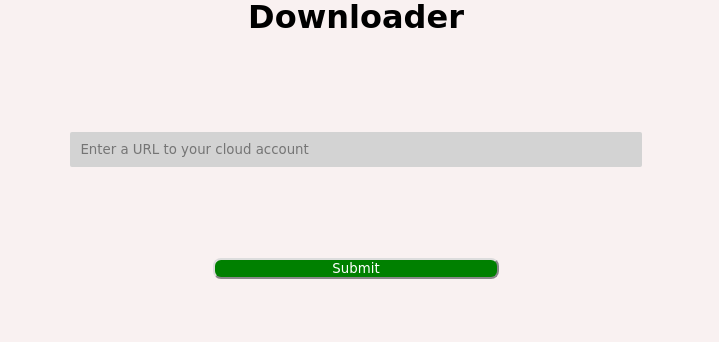
\includegraphics[scale=.7]{s0}
        \caption{First page, ready for a url to a cloud platform.}
    \end{figure}

    \begin{figure}[h]
    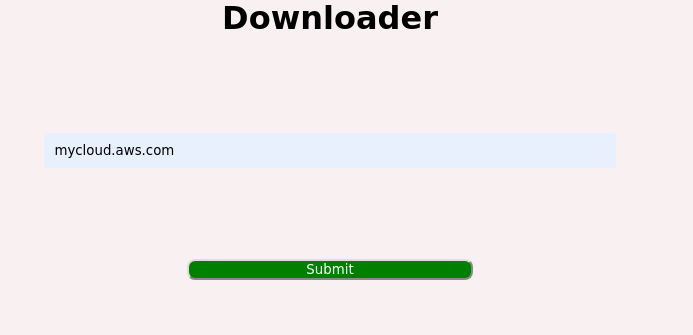
\includegraphics[scale=.7]{s1}
        \caption{URL entered that goes to cloud account.}
    \end{figure}

    \begin{figure}[h]
    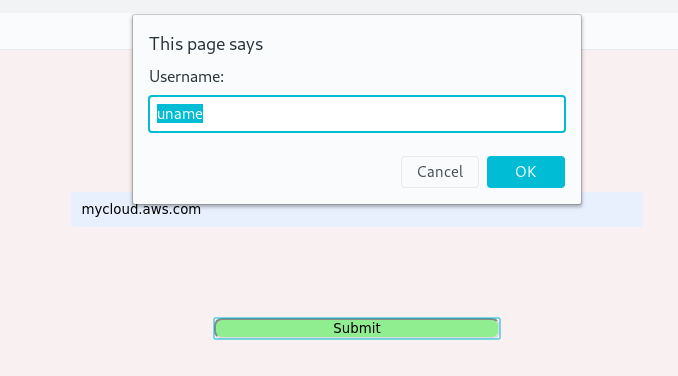
\includegraphics[scale=.7]{s2}
        \caption{Username to cloud platform entered.}
        \label{fig:clouduname}
    \end{figure}

    \begin{figure}[h]
    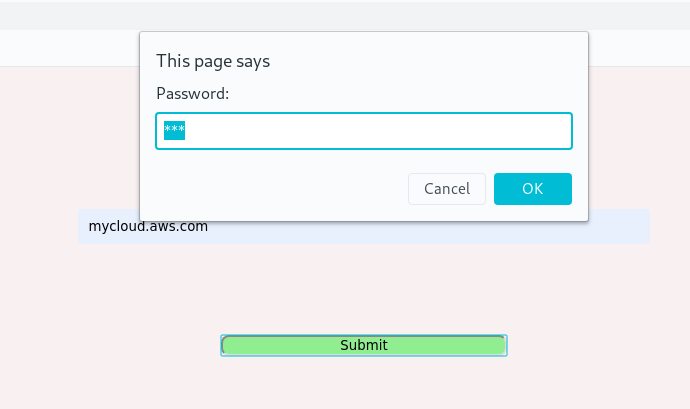
\includegraphics[scale=.7]{s3}
        \caption{Password to cloud platform entered. Note: Javascript doesn't allow for a popup with two text boxes in
        the same window or two windows at the same time. The actual implementation
        will include both the username and password entry boxes in the same popup window.}
        \label{fig:cloudpass}
    \end{figure}

    \begin{figure}[h]
    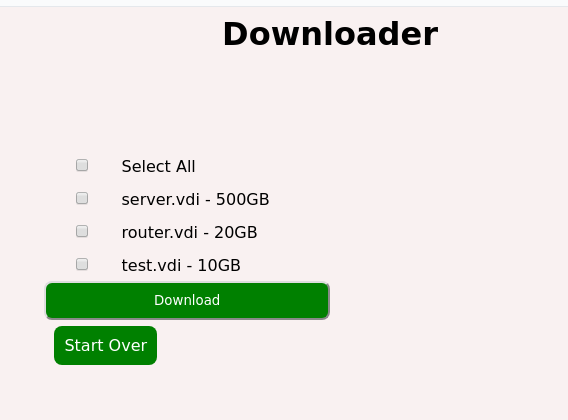
\includegraphics[scale=.7]{s4}
        \caption{Files available for downloading in the root directory of the cloud storage.}
    \end{figure}

    \begin{figure}[h]
    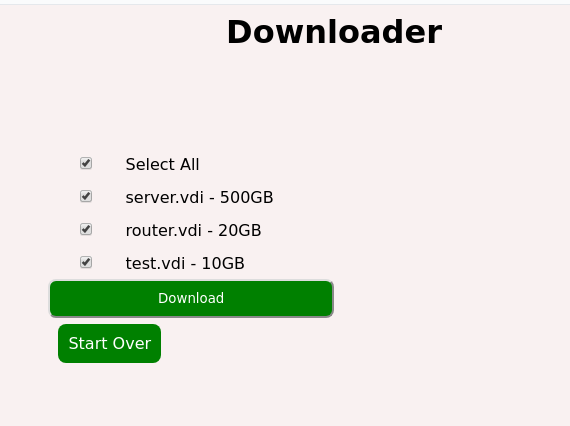
\includegraphics[scale=.7]{s5}
        \caption{All files selected for downloading.}
    \end{figure}

    \begin{figure}[h]
    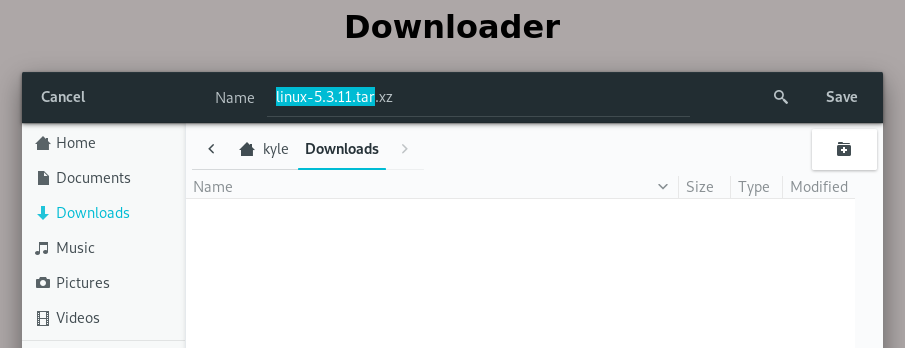
\includegraphics[scale=.5]{s6}
        \caption{Download button pressed, browser prompts where to save files.}
    \end{figure}

\end{document}
